\section{Computing the projection matrix}
One of the main problems when parallelizing the algorithm is that the amount of data in real applications is huge. Images from synchrotrons are generated with detectors of sizes up to about $4000\times4000$, with a typical detector size being about $2048\times2048$. To accurately generate 3D reconstructions it has been shown that approximately $\frac{\pi\cdot N}{2}$ vieweing angles are needed, where $N$ is the size of the detector in one direction~\cite{natterer2001}.\\
We benchmarked our algorithms by using sizes $N$ ranging from $128$ to $4096$ and using $\lceil\frac{\pi\cdot N}{2}\rceil$ angles and $N$ lines for each of these sizes to make the problem sizes realistic. However, in the future it might be worth investigating how the reconstructions look when using fewer angles, since one of the strengths of the SIRT algorithm is that it produces good results with few angles.\\
To solve the large problems it is not possible to store the whole system matrix on the GPU. Lets take as an example the amount of space used to store the matrix for a 3D problem with a $N=4000$ detector, with $\lceil\frac{\pi\cdot N}{2}\rceil$ angles, and $4000$ rays per angle. The matrix is sparse having at most $2\cdot N-1$ entries in each row, so instead of storing the whole matrix with all the zeroes, we will consider a semi-sparse representation with one 2 dimensional array containing the data as floats in arrays on each row of size  $2\cdot N-1$, and one matching 2 dimensional array containing the column indexes of the datapoints. This is also the representation we have used in our implementations. For the example sketched above the number of rows of each matrix will be $\lceil\frac{\pi\cdot4000}{2}\rceil\cdot4000$ and the number of columns is $2\cdot 4000-1$. Assuming ints and floats both take up 4 bytes each then storing the matrix requires $4\cdot 2\cdot\lceil\frac{ \pi \cdot 4000}{2} \rceil \cdot 4000 \cdot (2 \cdot 4000-1) \approx1TB$. This is of course one of the largest problems, but even for a problem with $N=512$ we're looking at the matrix taking up around $3-4GB$. Besides the matrix we also need to store the sinogram data which will take approximately $420MB$, and the reconstruction taking up around $270MB$. Hence even for relatively small problems we're looking at an estimated $5GB$ of data. GPU memory is expensive, and is typically in the range 2-8GB for consumer end cards, and 10-48GB for high end cards. Thus, the small problems are not able to fit in a standard comsumer card, and large problems won't fit on any cards. When we tested our algorithms, we were not able to copute the system matrix on the universities GPU's for sizes larger than $256\times256$.\todo{L\ae rke should probably check these calculations...}\\
There are several ways of getting around this problem. Some problems exhibit symmetries in the system matrix so that we only have to store part of the matrix. This is already somewhat accounted for in the above calculations. In the example we only considered the matrix for one slice of a 3D reconstruction since it will be equivalent for other slices when using parallel beam geometry. Thus for cone beam geometries, the memory needed would be approximately $N$ times greater. Other symetries involve angle symmetries, where for example a scan from a $45^{\circ}$ or $135^{\circ}$ angle would contain the same values for mirrored pixels. However these are obviously not generally applicable since they will depend on which angles are used in the reconstruction.\\
Another more flexible approach is to calculate the system matrix in chunks which is what we have done. For this we started by using the code from a bachelor project in which they did an implementation of finding the system matrix using futhark. We had two different parallel implementations in futhark and a sequential version in python which we compared. The sequential version in python was too slow (in the order of hours) for realistic problem sizes to be worth considering. When we compared the two bachelor projects one seemed to outperform the other both in terms of memory usage and computation time. Since one of the implementations ran in to problems with memory for some of the smallest problems, we decided to keep working with the most promising of the two. We call this algorithm \emph{projectionmatrix\_jh}.\\
The system matrix may be adequately approximated by considering the x-rays as being thin lines and calculating the length of intersections with each pixel in a grid. For simplicity we have only considered square grids with isotropic pixels.\\
\begin{figure}[h]
\begin{lstlisting}[frame=single]
for ray = 0; ray < numberofrays; ray++ //parallel
	for pixel = 0; pixel < pixels; pixel++ //parallel
		if ray intersects pixel:
        (p1,p2) = intersectionpoints pixel ray
        A[ray][pixel] = distance p1 p2
\end{lstlisting}
\label{sysmat}
  \caption{A looped version of the projection matrix algorithm.}
\end{figure}
The computation of the system matrix contains two levels of possible parallelization. The implementation from the bachelor project we used had parallelized over the outer loop - i.e for each ray. To compute the intersection lengths a sequential loop was run following each line. The number of rays is very high ($6.586.368$ for a grid of size $2048*2048$), and larger than the number of pixels, this seems a good choice. By following each line, the inner loop only runs $2*N-1$ times. From their report it seems they tried a naive implementation of computing the intersection with each pixel in parallel (akin to the pseudocode in ~\ref{sysmat}) but found it to be too slow to consider.\\
However, when we had an implementation of the foward projection and analyzed the compiled code, we could clearly see that the most time was spend in the kernel consisting of the sequential loop doing grid line intersections. Therefore we decided to spend some more time on the system matrix computations. Futhark does a lot of optimizations, but can not merge code across a loop in a map so our first approach was to attempt to change the inner loop to a map. However, since the inner loop is inherently sequential because of cross loop dependencies, we did not completely succeed. We seperated out the part of the code which computes the intersection point, and did the distance calculations as a map. We call this algorithm \emph{projectionmatrix\_map}.
Another issue with the projectionmatrix\_jh is a lot of branches in the inner loop. We also tried to limit the computations in these branches as much as possible in projectionmatrix\_map.\\
Since we did not manage to convert the inner loop to a map in projectionmatrix\_jh, we also attemted a different approach, explained in~\cite{Gao2012}. It is based on the observation that each line with slope at most $1$ intersects at most two rows of the grid in each column of the grid, and opposite for the lines with slope greater than $1$. Hence there is potential for exploiting a second level of parallelism by parrallelizing over the columns or rows of the grid and finding the nontrivial intersections. They show a method for doing this in time $O(1)$. Unfortunately there is a small bug somewhere our implementation which seems to be related to the transition between lines with slope $>1$ and those with slope $<1$. We did not manage to find the error, but have decided to include the algorithm in the benchmarking anyway, since we believe it is a small error somewhere with no significant influence of the speed of the algorithm. We call this algorithm \emph{projectionmatrix\_doubleparallel}.\\
\begin{figure}[h]
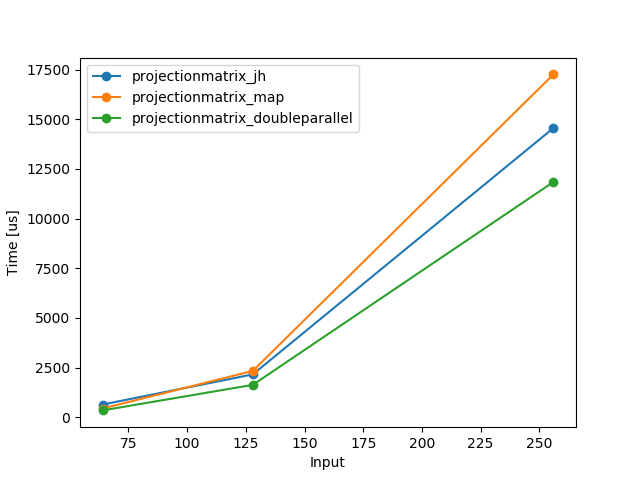
\includegraphics{images/resultsMatrixPlot.png}
\label{sysmatcompare}
  \caption{A lcomparison of the projection matrix algorithms run for gridsizes 64 to 256. Since the universities GPUs only have about 3GB of memory this was the largest size we could run for without chunking up the matrix.}
\end{figure}
We benchmarked the algorithms by generating the input, saving it to files and running with futhatk-bench. We used the opencl compiler, and did 10 runs. From the plot~\ref{sysmatcompare} we can see that the version where we exploit inner parallelism is indeed fastest. For the maximum size we were able to run, i.e 256 we got a speedup of about $1.2$ compared to projectionmatrix\_jh.
